\chapter{A combustão: combustíveis, produtos e gases de efeito estufa}\label{ch:g8:combustion-and-fuels}

Uma família dorme num apartamento cujo aquecedor a gás está com a
chaminé entupida. A chama, sem \omterm{def:g4:air-a-mixture-of-gases:air}{ar} suficiente, \omterm{def:g4:what-a-fire-needs:burning}{queima} mal, e um gás
invisível e sem cheiro vai enchendo devagar os cômodos. Às duas da
manhã, uma caixinha na parede começa a apitar: o detector de monóxido de
carbono. Todo mundo sai a tempo. O mesmo \omterm{def:g4:what-a-fire-needs:fuel}{combustível}, queimando bem, só
dá dióxido de carbono e água --- e esse dióxido de carbono tem a sua
própria história, escrita no \omterm{def:g4:air-a-mixture-of-gases:air}{ar} do planeta inteiro.

\begin{recall}
Uma \omterm{def:g4:what-a-fire-needs:burning}{queima}, ou \omterm{def:g4:what-a-fire-needs:burning}{combustão}, precisa de um \omterm{def:g4:what-a-fire-needs:fuel}{combustível}, de oxigênio e de
calor, e fabrica substâncias novas (\cref{ch:g4:what-a-fire-needs}). O
\omterm{def:g4:air-a-mixture-of-gases:air}{ar} tem cerca de um quinto de oxigênio
(\cref{ch:g4:air-a-mixture-of-gases}). Uma equação está balanceada
quando cada tipo de \omterm{def:g7:atoms-and-molecules:atom}{átomo} aparece o mesmo número de vezes dos dois lados
(\cref{ch:g8:balanced-equations}).
\end{recall}

\section{A queima do carbono e do metano}

\begin{example}[Duas combustões]\label{ex:g8:combustion-and-fuels:two}
O carbono (carvão vegetal, carvão mineral) \omterm{def:g4:what-a-fire-needs:burning}{queima} e dá dióxido de
carbono:
\[
  \ce{C(s) + O2(g) -> CO2(g)}.
\]
O metano, a parte principal do gás natural, \omterm{def:g4:what-a-fire-needs:burning}{queima} e dá dióxido de
carbono e água:
\[
  \ce{CH4(g) + 2O2(g) -> CO2(g) + 2H2O(l)}.
\]
Nos dois casos, a água de cal fica leitosa com o gás formado; com o
metano, um copo frio também fica embaçado.
\end{example}

\begin{method}[Escrever a combustão de um combustível feito de carbono e hidrogênio]\label{met:g8:combustion-and-fuels:write}
Para um \omterm{def:g4:what-a-fire-needs:fuel}{combustível} cujas \omterm{def:g7:atoms-and-molecules:molecule}{moléculas} contêm só carbono e hidrogênio:
\begin{enumerate}
  \item os produtos são o dióxido de carbono e a água;
  \item balanceie o carbono com \ce{CO2}, depois o hidrogênio com
        \ce{H2O};
  \item conte os \omterm{def:g7:atoms-and-molecules:atom}{átomos} de oxigênio à direita e balanceie-os com
        \ce{O2}; dobre tudo se aparecer uma metade.
\end{enumerate}
Para o butano: \ce{2C4H10 + 13O2 -> 8CO2 + 10H2O}.
\end{method}

\section{Combustão completa e incompleta}

\begin{definition}[Combustão completa e incompleta]\label{def:g8:combustion-and-fuels:complete}
Uma \emph{combustão completa}\index{combustao completa@combustão completa} acontece com
oxigênio suficiente: todo o carbono do \omterm{def:g4:what-a-fire-needs:fuel}{combustível} vira dióxido de
carbono. Uma \emph{combustão incompleta}\index{combustao incompleta@combustão incompleta}
acontece com pouco oxigênio: uma parte do carbono vira monóxido de
carbono, \ce{CO}, ou fuligem, que é carbono, \ce{C}.
\end{definition}

\begin{example}[O metano com falta de oxigênio]\label{ex:g8:combustion-and-fuels:incomplete}
Com pouco \omterm{def:g4:air-a-mixture-of-gases:air}{ar}, o metano pode queimar dando monóxido de carbono ou
fuligem:
\[
  \ce{2CH4 + 3O2 -> 2CO + 4H2O}, \qquad \ce{CH4 + O2 -> C + 2H2O}.
\]
\end{example}

\begin{proposition}[Ler uma chama]\label{prop:g8:combustion-and-fuels:flame}
Um bico de Bunsen com a entrada de \omterm{def:g4:air-a-mixture-of-gases:air}{ar} aberta mistura \omterm{def:g4:air-a-mixture-of-gases:air}{ar} ao gás antes de
ele queimar: a chama é azul e quase invisível, a \omterm{def:g4:what-a-fire-needs:burning}{combustão} é completa.
Com a entrada de \omterm{def:g4:air-a-mixture-of-gases:air}{ar} fechada, o gás encontra pouco oxigênio: a chama é
amarela, fumacenta, e escurece de fuligem um objeto frio colocado nela
--- a \omterm{def:g4:what-a-fire-needs:burning}{combustão} é incompleta.
\end{proposition}

\begin{omfigure}
\begin{tikzpicture}[font=\small, scale=1.3]
  \pic[transform shape] at (0,0) {bunsen=open};
  \node[anchor=north, align=center] at (0,-0.1) {entrada de ar aberta:\\ chama azul, completa};
  \pic[transform shape] at (4,0) {bunsen=closed};
  \node[anchor=north, align=center] at (4,-0.1) {entrada de ar fechada:\\ chama amarela, incompleta};
  \draw[<-, omProp, thick] (0.08,0.6) -- (1.4,0.9) node[right, text=black] {entrada de ar};
  \draw[<-, omProp, thick] (-0.4,0.3) -- (-1.3,0.6) node[left, text=black] {gás};
  \draw[<-, omProp, thick] (4.15,3.3) -- (5.0,3.5) node[right, text=black, align=left]
    {fuligem, monóxido\\ de carbono};
\end{tikzpicture}

{\small Um bico de Bunsen. O \omterm{def:g4:air-a-mixture-of-gases:air}{ar} que entra por baixo dá uma chama azul e
uma \omterm{def:g8:combustion-and-fuels:complete}{combustão completa}; sem ele, a chama é amarela e fumacenta.}
\end{omfigure}

\begin{omfigure}
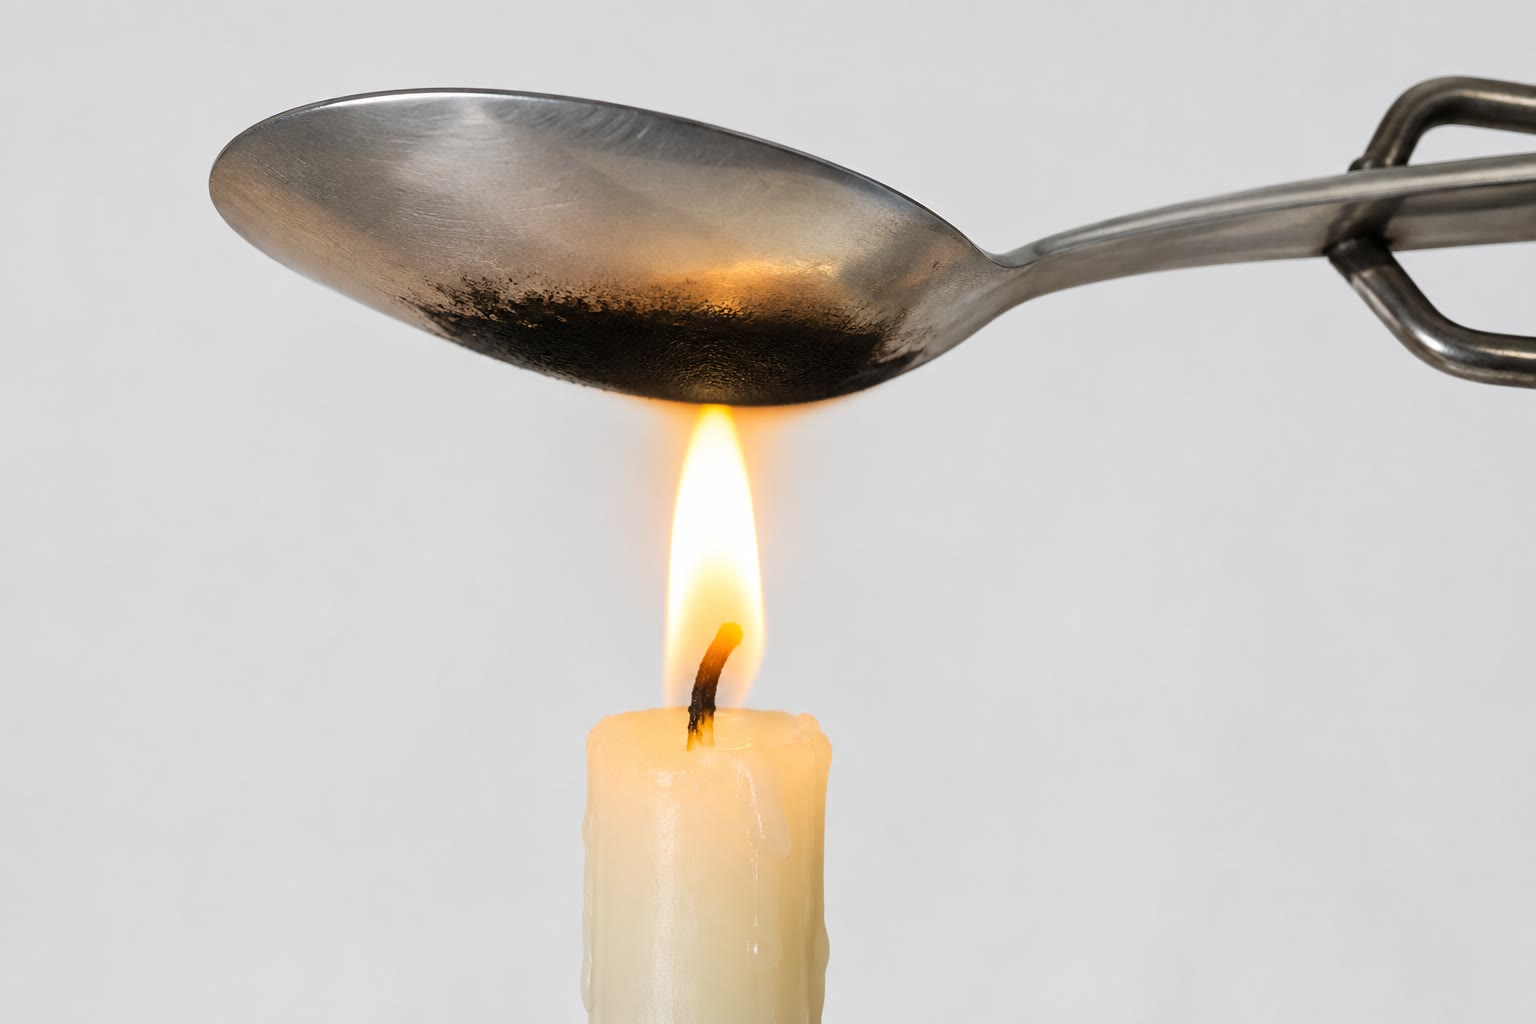
\includegraphics[width=0.45\linewidth]{images/book1/ai/g8-soot-spoon.jpg}

{\small Uma colher fria segurada na chama amarela de uma vela fica preta
de fuligem: a \omterm{def:g4:what-a-fire-needs:burning}{combustão} é incompleta.}
\end{omfigure}

\section{O monóxido de carbono, um perigo silencioso}

\begin{proposition}[Por que o monóxido de carbono mata]\label{prop:g8:combustion-and-fuels:co}
O monóxido de carbono não tem cor, nem cheiro, nem gosto. Inspirado, ele
toma o lugar do oxigênio no sangue (o livro de biologia explica como),
provocando dor de cabeça, sonolência e, num cômodo fechado, perda de
consciência e morte. Ele é produzido por qualquer \omterm{def:g4:what-a-fire-needs:fuel}{combustível} que \omterm{def:g4:what-a-fire-needs:burning}{queima}
com falta de \omterm{def:g4:air-a-mixture-of-gases:air}{ar}: uma caldeira ou um aquecedor a gás com manutenção ruim
ou com a chaminé entupida, um fogareiro numa barraca fechada, uma
churrasqueira ou um gerador usados dentro de casa.
\end{proposition}

\begin{safety}{\ghs[0.8cm]{GHS02}\ghs[0.8cm]{GHS04}\ghs[0.8cm]{GHS06}\ghs[0.8cm]{GHS08}}
% ledger: ghs:CO
Monóxido de carbono: gás extremamente inflamável (GHS02), fornecido sob
pressão (GHS04); tóxico se inalado (GHS06); afeta os órgãos por
exposição repetida e pode prejudicar o feto (GHS08).
\end{safety}

\begin{remark}[Prevenir a intoxicação]\label{rem:g8:combustion-and-fuels:prevent}
Os aparelhos a gás passam por manutenção regular feita por um
profissional, as chaminés e as aberturas de ventilação nunca são
obstruídas, as churrasqueiras e os geradores só são usados ao \omterm{def:g4:air-a-mixture-of-gases:air}{ar} livre,
e um detector de monóxido de carbono é instalado perto de qualquer
queimador.
\end{remark}

\begin{omfigure}
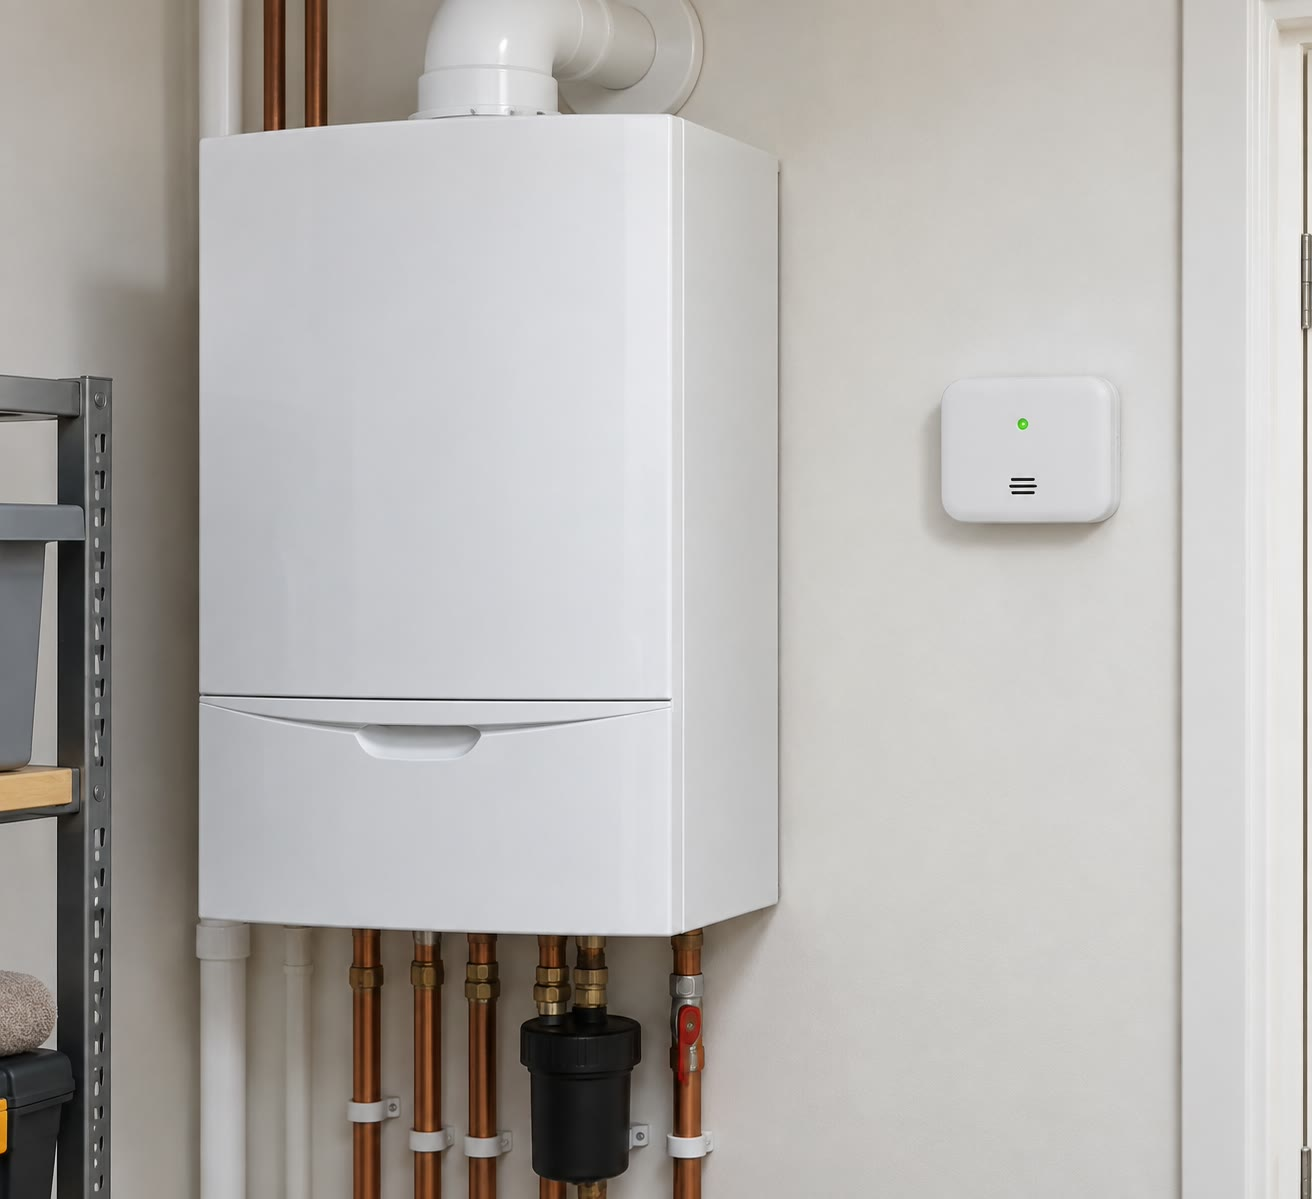
\includegraphics[width=0.45\linewidth]{images/book1/ai/g8-boiler-alarm.jpg}

{\small Uma caldeira a gás e, ao lado dela, um detector de monóxido de
carbono.}
\end{omfigure}

\section{O dióxido de carbono e o efeito estufa}

\begin{definition}[Gás de efeito estufa]\label{def:g8:combustion-and-fuels:greenhouse}
Um \emph{gás de efeito estufa}\index{gas de efeito estufa@gás de efeito estufa} é um gás do
\omterm{def:g4:air-a-mixture-of-gases:air}{ar} que deixa passar a luz do Sol, mas retém uma parte do calor que a
superfície da Terra devolve para o espaço, e assim aquece a parte baixa
da atmosfera. O vapor de água, o dióxido de carbono e o metano são gases
de efeito estufa; o nitrogênio e o oxigênio não são. (Como isso
acontece é explicado no livro de física.)
\end{definition}

\begin{proposition}[O dióxido de carbono do ar está aumentando]\label{prop:g8:combustion-and-fuels:rising}
% ledger: co2:mlo-1959, co2:mlo-2025 (rise 111.4 ppm, +35 %)
A quantidade de dióxido de carbono no \omterm{def:g4:air-a-mixture-of-gases:air}{ar} é medida sem interrupção desde
1959 num observatório no alto de uma montanha, no meio do oceano
Pacífico. Ela era de 316 partes por milhão (ppm) de \omterm{def:g4:air-a-mixture-of-gases:air}{ar} em 1959 e de 427
ppm em 2025: um aumento de cerca de \qty{35}{\percent} no tempo de uma
vida humana, causado principalmente pela \omterm{def:g4:what-a-fire-needs:burning}{queima} de carvão, petróleo e
gás natural. O dióxido de carbono a mais reforça o efeito estufa e
aquece o clima.
\end{proposition}

\begin{omfigure}
\begin{tikzpicture}
\begin{axis}[width=0.85\linewidth, height=6cm, xmin=1955, xmax=2030,
    ymin=300, ymax=440, xlabel={ano}, ylabel={dióxido de carbono (ppm)},
    axis lines*=left, ymajorgrids, grid style={gray!20},
    tick label style={font=\small, /pgf/number format/1000 sep={}},
    label style={font=\small}]
\addplot[omDef, thick, mark=*, mark size=0.8pt]
  table[x=year, y=ppm] {figdata/out/grade-8-co2-record.dat};
\node[anchor=west, font=\small] at (axis cs:1962,306) {316 ppm em 1959};
\node[anchor=east, font=\small] at (axis cs:2023,428) {427 ppm em 2025};
\end{axis}
\end{tikzpicture}

{\small Média anual do dióxido de carbono no \omterm{def:g4:air-a-mixture-of-gases:air}{ar}, medida desde 1959
(dados do NOAA Global Monitoring Laboratory; antes de 1974, da Scripps
Institution of Oceanography).}
\end{omfigure}

\section{Combustíveis fósseis e renováveis}

\begin{definition}[Combustíveis fósseis e renováveis]\label{def:g8:combustion-and-fuels:fossil}
Um \emph{combustível fóssil}\index{combustivel fossil@combustível fóssil} --- o carvão
mineral, o petróleo, o gás natural --- se formou no subsolo ao longo de
milhões de anos, a partir dos restos de plantas e de organismos
marinhos antigos. Um \emph{combustível renovável}\index{combustivel renovavel@combustível renovável}
é produzido a partir de plantas cultivadas hoje, ou de
resíduos: a lenha, o biogás de esterco e de restos de comida, o etanol
feito de beterraba ou de cana-de-açúcar.
\end{definition}

\begin{proposition}[De onde vem o carbono]\label{prop:g8:combustion-and-fuels:cycle}
As plantas tiram dióxido de carbono do \omterm{def:g4:air-a-mixture-of-gases:air}{ar} para crescer. Queimar um
\omterm{def:g8:combustion-and-fuels:fossil}{combustível renovável} devolve o dióxido de carbono que as plantas dele
tiraram do \omterm{def:g4:air-a-mixture-of-gases:air}{ar} há poucos anos. Queimar um \omterm{def:g8:combustion-and-fuels:fossil}{combustível fóssil} libera um
carbono que estava guardado no subsolo havia milhões de anos: isso
acrescenta dióxido de carbono ao \omterm{def:g4:air-a-mixture-of-gases:air}{ar}.
\end{proposition}

\begin{omfigure}
\begin{tikzpicture}[font=\small,
    box/.style={draw=omDef, fill=omDef!6, rounded corners=2pt, align=center,
      minimum height=0.9cm, text width=2.6cm}]
  \node[box] (air) at (0,3) {dióxido de\\ carbono no ar};
  \node[box] (plants) at (5.6,3) {plantas crescem\\ (tiram \ce{CO2})};
  \node[box] (fuel) at (5.6,0.4) {lenha, biogás,\\ bioetanol};
  \node[box, draw=black!50, fill=black!8] (fossil) at (0,0.4) {carvão, petróleo,\\ gás: no subsolo};
  \draw[->, thick, omProp] (air) -- (plants);
  \draw[->, thick, omProp] (plants) -- (fuel);
  \draw[->, thick, omProp] (fuel) -- (air);
  \node[text=black, font=\footnotesize, align=left, anchor=north west] at (1.5,1.45)
    {queima, poucos\\ anos depois};
  \draw[->, thick, black!60] (fossil) -- node[midway, left, text=black, font=\footnotesize,
    align=right] {queima: carbono\\ guardado por\\ milhões de anos} (air);
\end{tikzpicture}

{\small Os \omterm{def:g8:combustion-and-fuels:fossil}{combustíveis renováveis} devolvem ao \omterm{def:g4:air-a-mixture-of-gases:air}{ar} o carbono que as plantas
deles tiraram dele; os \omterm{def:g8:combustion-and-fuels:fossil}{combustíveis fósseis} acrescentam um carbono que
estava guardado no subsolo.}
\end{omfigure}

\begin{omfigure}
\begin{minipage}[t]{0.48\linewidth}\centering
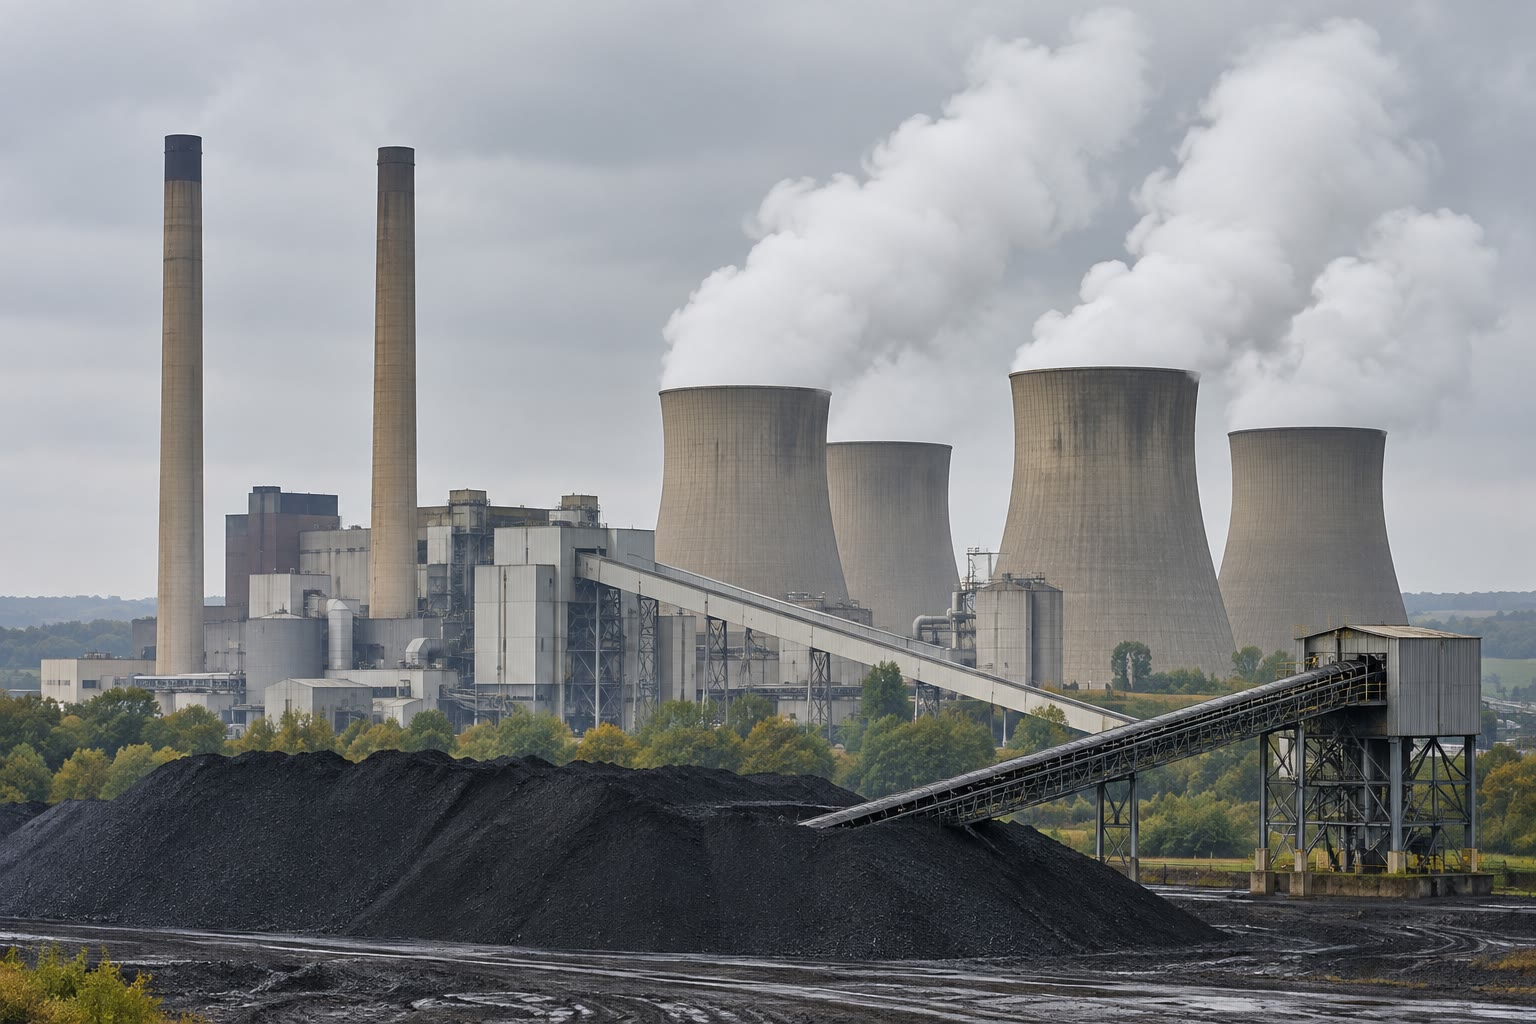
\includegraphics[width=\linewidth,height=4.6cm,keepaspectratio]{images/book1/ai/g8-coal-plant.jpg}

{\small Uma usina termelétrica a carvão.}
\end{minipage}\hfill
\begin{minipage}[t]{0.48\linewidth}\centering
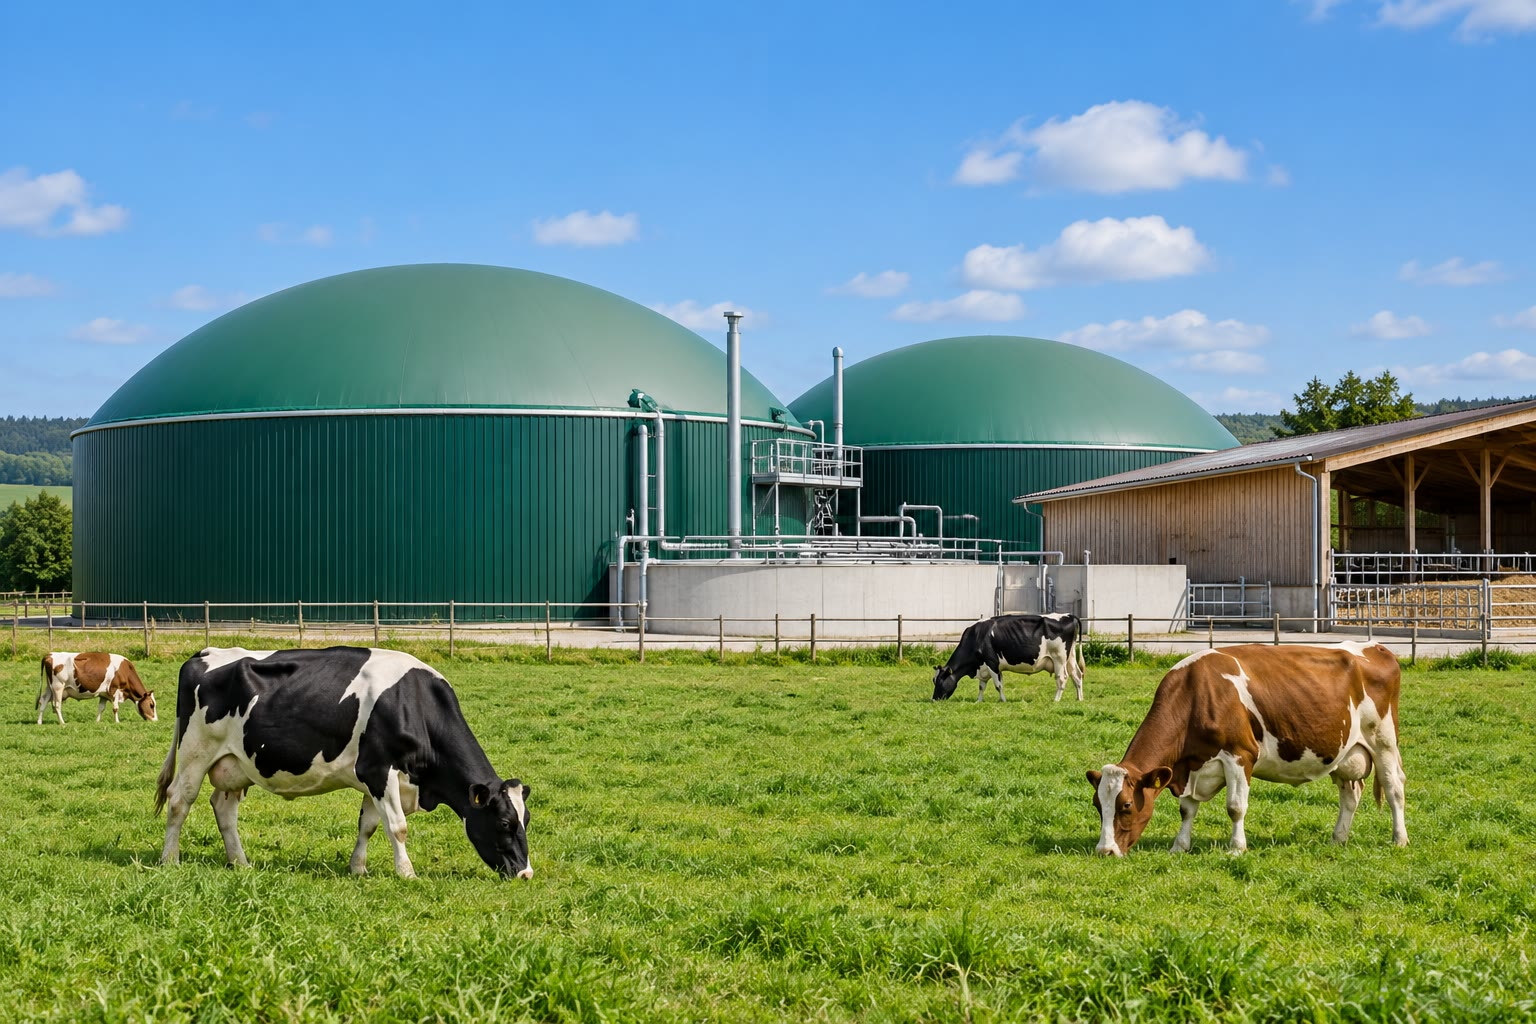
\includegraphics[width=\linewidth,height=4.6cm,keepaspectratio]{images/book1/ai/g8-biogas-farm.jpg}

{\small Uma usina de biogás numa fazenda: o esterco vira um \omterm{def:g8:combustion-and-fuels:fossil}{combustível renovável}.}
\end{minipage}
\end{omfigure}

\section{Exercícios}

\begin{exercise}[$\star$]\label{exo:g8:combustion-and-fuels:1}
Escreva a \omterm{def:g8:balanced-equations:equation}{equação balanceada} da \omterm{def:g8:combustion-and-fuels:complete}{combustão completa} do carbono.
\end{exercise}

\begin{exercise}[$\star$]\label{exo:g8:combustion-and-fuels:2}
Qual é a diferença entre uma \omterm{def:g8:combustion-and-fuels:complete}{combustão completa} e uma \omterm{def:g8:combustion-and-fuels:complete}{combustão
incompleta}?
\end{exercise}

\begin{exercise}[$\star$]\label{exo:g8:combustion-and-fuels:3}
Por que o monóxido de carbono é chamado de perigo silencioso?
\end{exercise}

\begin{exercise}[$\star$]\label{exo:g8:combustion-and-fuels:4}
Fóssil ou renovável: carvão mineral, lenha, gás natural, biogás,
gasolina, etanol de beterraba?
\end{exercise}

\begin{exercise}[$\star\star$]\label{exo:g8:combustion-and-fuels:5}
Escreva a \omterm{def:g8:balanced-equations:equation}{equação balanceada} da \omterm{def:g8:combustion-and-fuels:complete}{combustão completa} do propano,
\ce{C3H8}.
\end{exercise}

\begin{exercise}[$\star\star$]\label{exo:g8:combustion-and-fuels:6}
O etanol, \ce{C2H6O}, \omterm{def:g4:what-a-fire-needs:burning}{queima} completamente no oxigênio. Balanceie
\ce{C2H6O + O2 -> CO2 + H2O}. % ce-unbalanced-ok (to balance)
\end{exercise}

\begin{exercise}[$\star\star$]\label{exo:g8:combustion-and-fuels:7}
Uma panela colocada sobre uma chama amarela fica preta por baixo. Qual é
a substância preta? O que ela nos diz sobre a \omterm{def:g4:what-a-fire-needs:burning}{combustão}?
\end{exercise}

\begin{exercise}[$\star\star$]\label{exo:g8:combustion-and-fuels:8}
Leia a curva do dióxido de carbono: mais ou menos quanto dióxido de
carbono o \omterm{def:g4:air-a-mixture-of-gases:air}{ar} continha em 1980 e em 2000? Quantos ppm ele subiu nesses
vinte anos?
\end{exercise}

\begin{exercise}[$\star\star$]\label{exo:g8:combustion-and-fuels:9}
Por que queimar lenha acrescenta menos dióxido de carbono ao \omterm{def:g4:air-a-mixture-of-gases:air}{ar}, ao
longo dos anos, do que queimar carvão mineral, embora os dois deem
dióxido de carbono?
\end{exercise}

\begin{exercise}[$\star\star$]\label{exo:g8:combustion-and-fuels:10}
Balanceie a \omterm{def:g8:combustion-and-fuels:complete}{combustão incompleta} do carbono em monóxido de carbono,
\ce{C + O2 -> CO}. % ce-unbalanced-ok (to balance)
\end{exercise}

\begin{exercise}[$\star\star\star$]\label{exo:g8:combustion-and-fuels:11}
De 1959 (316 ppm) a 2025 (427 ppm), em que porcentagem o dióxido de
carbono do \omterm{def:g4:air-a-mixture-of-gases:air}{ar} aumentou? Arredonde para o número inteiro mais próximo.
\end{exercise}

\begin{exercise}[$\star\star\star$]\label{exo:g8:combustion-and-fuels:12}
Um aquecedor a gás é usado num quarto pequeno com a janela fechada.
Explique, usando duas equações deste capítulo, como a \omterm{def:g4:what-a-fire-needs:burning}{combustão} pode
passar de completa a incompleta com o tempo, e por que isso é perigoso.
\end{exercise}

\section{Problema: o fogareiro na barraca}

\begin{problem}[{Problema de fim de semana --- um fogareiro de camping, o
gás que ele queima, o que ele produz e por que ele nunca entra numa
barraca}]
\label{pb:g8:combustion-and-fuels:1}
% ledger: ghs:propane
Um fogareiro de camping \omterm{def:g4:what-a-fire-needs:burning}{queima} propano, \ce{C3H8}, de um cartucho que
contém \qty{450}{g} dele. Ao \omterm{def:g4:air-a-mixture-of-gases:air}{ar} livre, a chama é azul. Use estas
proporções em massa, tiradas da \omterm{def:g8:balanced-equations:equation}{equação balanceada}: \qty{44}{g} de
propano que queimam completamente dão \qty{132}{g} de dióxido de
carbono.

\medskip
\noindent\textbf{Parte I --- As equações.}
\begin{enumerate}
  \item Escreva a \omterm{def:g8:balanced-equations:equation}{equação balanceada} da \omterm{def:g8:combustion-and-fuels:complete}{combustão completa} do propano.
  \item Verifique-a contando os \omterm{def:g7:atoms-and-molecules:atom}{átomos} de cada tipo de cada lado.
  \item Balanceie a \omterm{def:g8:combustion-and-fuels:complete}{combustão incompleta}
        \ce{C3H8 + O2 -> CO + H2O}. % ce-unbalanced-ok (to balance)
  \item Qual das duas precisa de mais oxigênio por \omterm{def:g7:atoms-and-molecules:molecule}{molécula} de propano?
\end{enumerate}

\medskip
\noindent\textbf{Parte II --- Dentro de uma barraca.}
\begin{enumerate}[resume]
  \item Um fogareiro aceso dentro de uma barraca fechada logo passa a
        queimar com uma chama amarela. Explique por quê.
  \item Que gás perigoso se forma então? Dê duas propriedades dele que o
        tornam difícil de perceber.
  \item O cartucho de propano traz dois pictogramas. Dê o nome deles e
        diga o que cada um significa.
  \item Dê duas regras para usar um fogareiro de camping com segurança.
\end{enumerate}

\medskip
\noindent\textbf{Parte III --- O dióxido de carbono de um cartucho.}
\begin{enumerate}[resume]
  \item Quantas vezes o dióxido de carbono formado é mais pesado do que o
        propano queimado?
  \item De onde vêm os gramas a mais?
  \item O propano é um \omterm{def:g8:combustion-and-fuels:fossil}{combustível fóssil} ou renovável? Queimá-lo
        acrescenta dióxido de carbono ao \omterm{def:g4:air-a-mixture-of-gases:air}{ar}?
  \item Calcule a massa de dióxido de carbono liberada quando um cartucho
        inteiro de \qty{450}{g} \omterm{def:g4:what-a-fire-needs:burning}{queima} completamente.
\end{enumerate}
\end{problem}
